\documentclass[10pt,leter,openany]{article}
\usepackage[latin1]{inputenc}
\usepackage[english]{babel}
\usepackage{amsmath}
\usepackage{amsfonts}
\usepackage{amssymb}
\usepackage{graphicx}
\usepackage{listings}
\usepackage{color}
\usepackage[left=3cm,right=3cm,top=3cm,bottom=3cm]{geometry}
\usepackage[numbers,sort&compress]{natbib}
\usepackage{url}
\usepackage{caption}
\usepackage{siunitx}
\usepackage{subfigure}
\usepackage{float}
\usepackage{booktabs}

\usepackage{comment}

\setlength{\parindent}{0pt}
\setlength{\parskip}{4pt}

\definecolor{mygreen}{rgb}{0,0.6,0}
\definecolor{mygray}{rgb}{0.5,0.5,0.5}
\definecolor{mymauve}{rgb}{0.58,0,0.82}

\lstset{ 
	backgroundcolor=\color{white},   % choose the background color; you must add \usepackage{color} or \usepackage{xcolor}; should come as last argument
	basicstyle=\footnotesize,        % the size of the fonts that are used for the code
	breakatwhitespace=false,         % sets if automatic breaks should only happen at whitespace
	breaklines=true,                 % sets automatic line breaking
	captionpos=b,                    % sets the caption-position to bottom
	commentstyle=\color{mygreen},    % comment style
	deletekeywords={...},            % if you want to delete keywords from the given language
	escapeinside={\%*}{*)},          % if you want to add LaTeX within your code
	extendedchars=true,              % lets you use non-ASCII characters; for 8-bits encodings only, does not work with UTF-8
	firstnumber=01,                	 % start line enumeration with line 1000
	frame=single,	                 % adds a frame around the code
	keepspaces=true,                 % keeps spaces in text, useful for keeping indentation of code (possibly needs columns=flexible)
	keywordstyle=\color{blue},       % keyword style
	language=Python,                 % the language of the code
	morekeywords={*,...},            % if you want to add more keywords to the set
	numbers=left,                    % where to put the line-numbers; possible values are (none, left, right)
	numbersep=5pt,                   % how far the line-numbers are from the code
	numberstyle=\tiny\color{mygray}, % the style that is used for the line-numbers
	rulecolor=\color{black},         % if not set, the frame-color may be changed on line-breaks within not-black text (e.g. comments (green here))
	showspaces=false,                % show spaces everywhere adding particular underscores; it overrides 'showstringspaces'
	showstringspaces=false,          % underline spaces within strings only
	showtabs=false,                  % show tabs within strings adding particular underscores
	stepnumber=1,                    % the step between two line-numbers. If it's 1, each line will be numbered
	stringstyle=\color{mymauve},     % string literal style
	tabsize=2,	                     % sets default tabsize to 2 spaces
	title=\lstname                   % show the filename of files included with \lstinputlisting; also try caption instead of title
}

\usepackage{titling}
\newcommand{\subtitle}[1]{%
	\posttitle{%
		\par\end{center}
	\begin{center}\large#1\end{center}
	\vskip0.5em}%
}


\author{5273}
\title{Homework Assignment 3: Applied Probabilistic Models}
\subtitle{Word Distributions}
\date{}



\begin{document}
	
\maketitle

\section{Introduction}
	
	For this work, data is collected on the free eBooks library Project Gutenberg \citep{gutenberg}. The chosen book for the analysis is: ``The Autobiography of Benjamin Franklin" \citep{franklin2007autobiography}. Data obtained from the Project Gutenberg are in \texttt{txt} format.
	
	For the analysis, it is used the R software in its version 4.0.2 \citep{r}, and the code used is available on the GitHub repository \citep{github}. This work is run on a MacBook Air with an Intel Core i5 CPU $ @ $ 1.8 GHz and 8 GB RAM.
	
\section{Data Distribution}
	 
	The book is downloaded directly from the web and in order to develop the analysis, the following code is used.
	
	\lstinputlisting[language=R, firstline=1, lastline=15]{a3.R}
	
	In this work, it is analyzed how frequencies of English words are distributed. The first discussed aspects are events that describe two known distributions. The second part corresponds to the other two events that can be worth finding which distribution best fits the data. For this last issue, it is recommended to see the paper of \citet{delignette2015fitdistrplus}.
	
\subsection{Geometric Distribution}
	Since the book is an autobiography it is redacted in the first person, so it is expected the word ``I" appears multiple times referring to facts corresponding to the author himself. Some statistics of this pronoun are studied. The first aspect to analyze is how many words have been used when the ``I" appears. This may correspond to a geometric distribution, which can be described as the number of repetitions resulting in failures until the first success is achieved. In this case, all the words written until the pronoun is used can be considered as failures, and the use of ``I" is the success. Figure \ref{fig:wordsforI} shows a histogram of how this aspect is represented in the book.
	
		\begin{figure}
		\begin{center}
			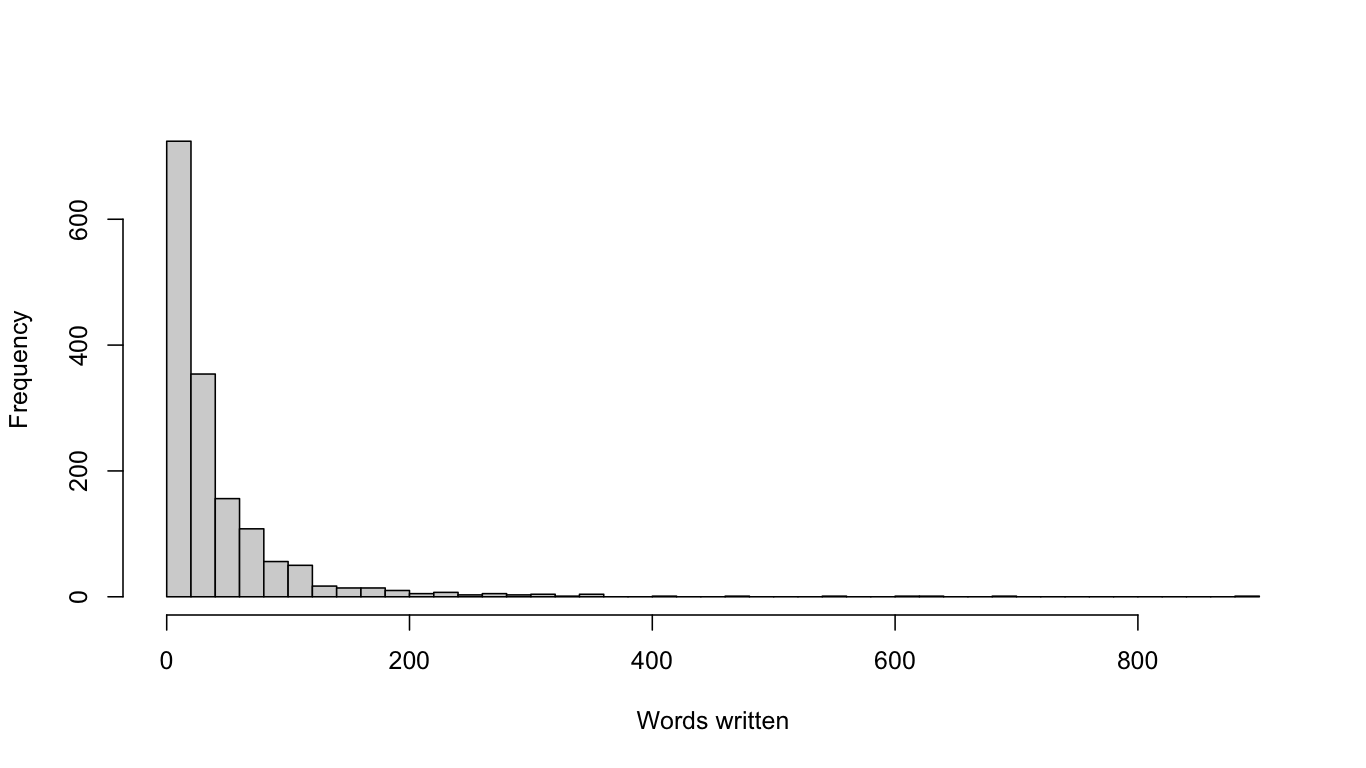
\includegraphics[scale=0.3]{img/words_forI}
			\captionof{figure}{Histogram of the amount of words used before the pronoun ``I"}
			\label{fig:wordsforI}
		\end{center}
	\end{figure}

\subsection{Binomial distribution}

	The number of times this pronoun is used in each sentence of the book is another event that could be analyzed. This case could be described as a binomial distribution, which describes the number of success obtained in $ n  $ Bernoulli repetitions. For this example, those repetitions are the total number of sentences in the text whereas the number of success is given by the presence of the pronoun ``I" in $ k $ times. This is shown in the histogram corresponding to Figure \ref{fig:numberofI}. 
	
	\begin{figure}
	\begin{center}
		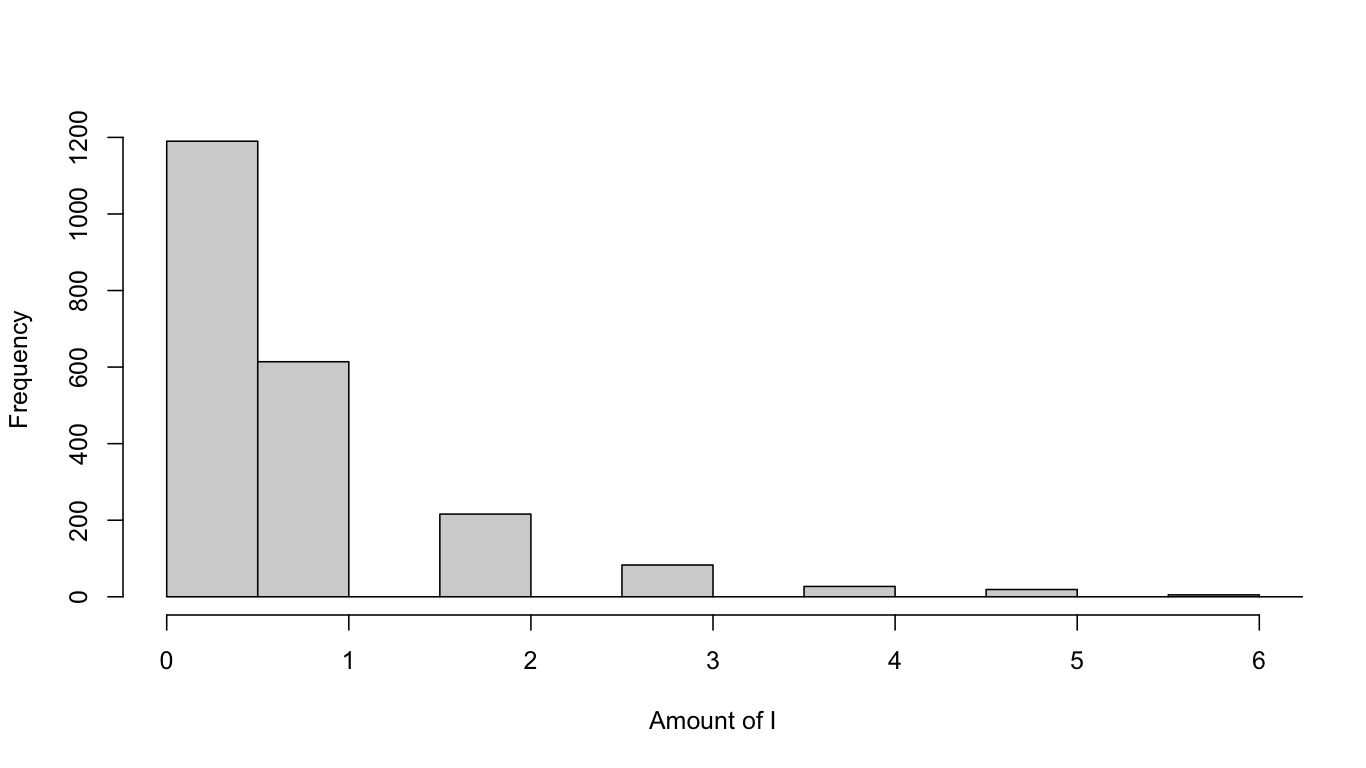
\includegraphics[scale=0.3]{img/number_of_I}
		\captionof{figure}{Histogram of the amount of times  the pronoun ``I" is mentioned in sentences}
		\label{fig:numberofI}
	\end{center}
\end{figure}

\subsection{Other distributions}

 Length of English words and also its quantity when constructing paragraphs are the other considered aspects. Figure \ref{fig:words1} shows a histogram of words length used throughout the book and Figure \ref{fig:words2} shows a histogram of the amount of word used per paragraph in the document. 
 
 Last, Figure \ref{fig:fit} show a skewness-kurtosis plot such as the one proposed by \citet{cullen1999probabilistic} for the empirical distribution of both events. In this plot, values for common distributions are displayed in order to help the choice of distributions to fit data. The distribution is represented by a single point on the plot. According to \citet{delignette2015fitdistrplus} skewness and kurtosis are known not to be robust, thus the plot should then be regarded as indicative only. A non-zero skewness reveals a lack of symmetry of the empirical distribution. For words length and words per paragraph, the skewness has values of 0.996 and 3.128 respectively.   The kurtosis value quantifies the weight of tails in comparison to the normal distribution for which the kurtosis equals 3. The values of kurtosis are 3.519 for word length and 27.017 for words per paragraph.

\begin{figure}
	\begin{center}
		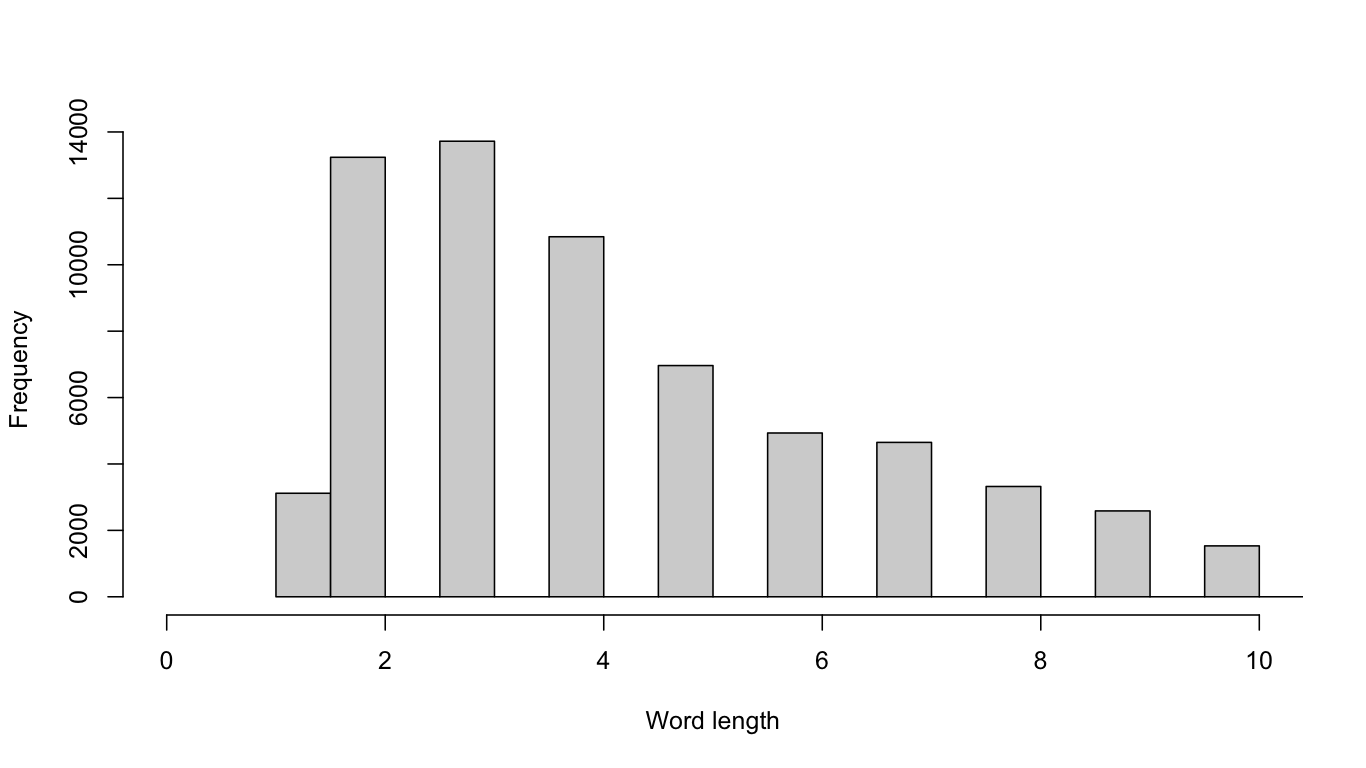
\includegraphics[scale=0.3]{img/word_lengths}
		\captionof{figure}{Histogram of lenght of words used in the book}
		\label{fig:words1}
	\end{center}
\end{figure}

\begin{figure}
	\begin{center}
		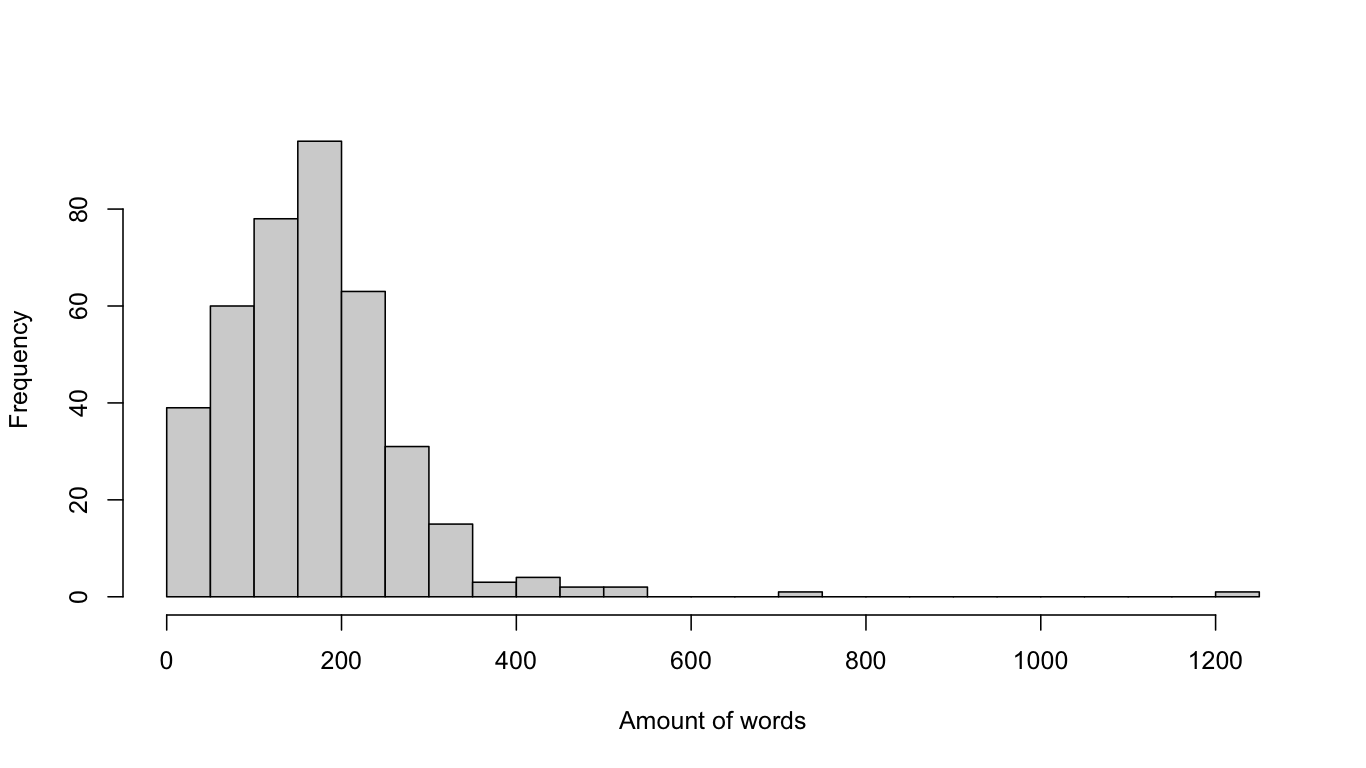
\includegraphics[scale=0.37]{img/word_amount}
		\captionof{figure}{Histogram of the amount of words used per paragraph}
		\label{fig:words2}
	\end{center}
\end{figure}


\begin{figure}
	\centering
	\subfigure[Cullen and Frey graph for words lenght present in the document]{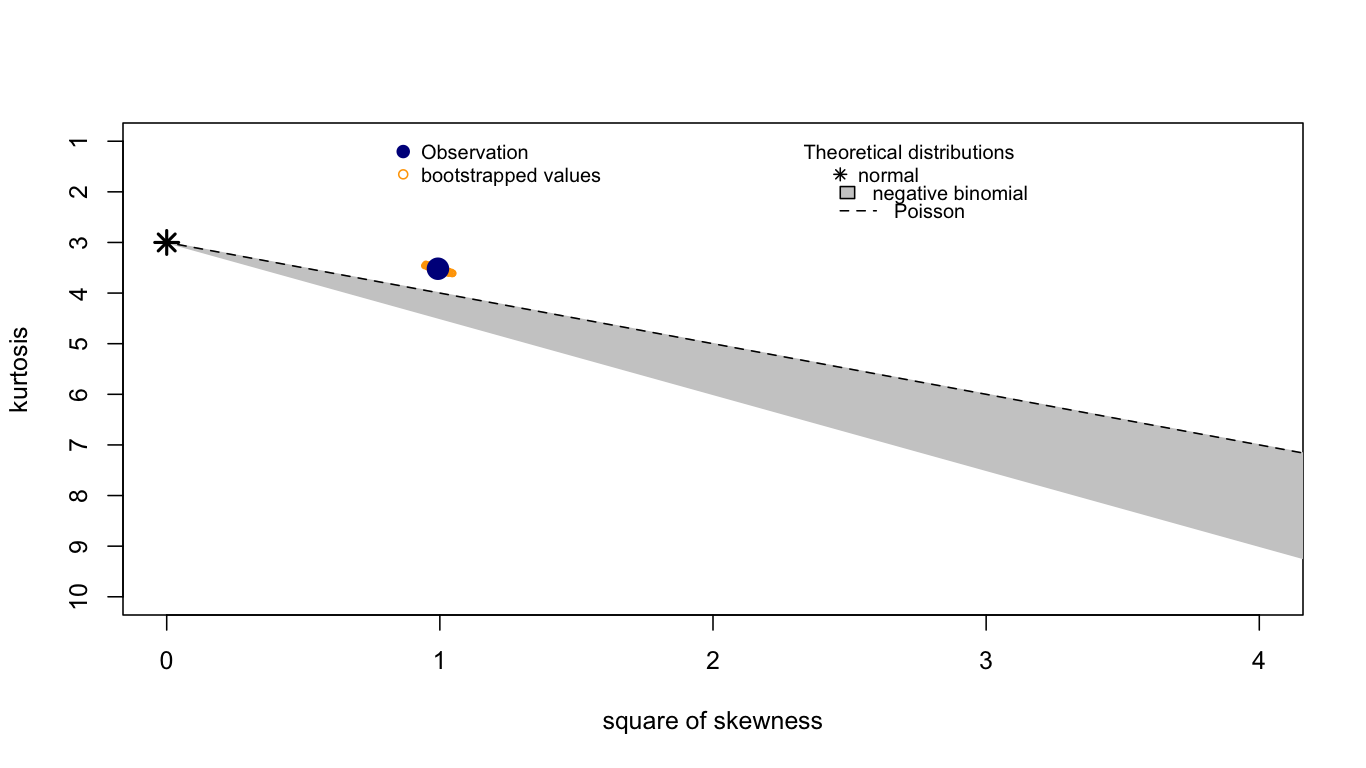
\includegraphics[width=170mm]{img/_fitofwordlenght}}
	\subfigure[Cullen and Frey graph for words per paragraphs]{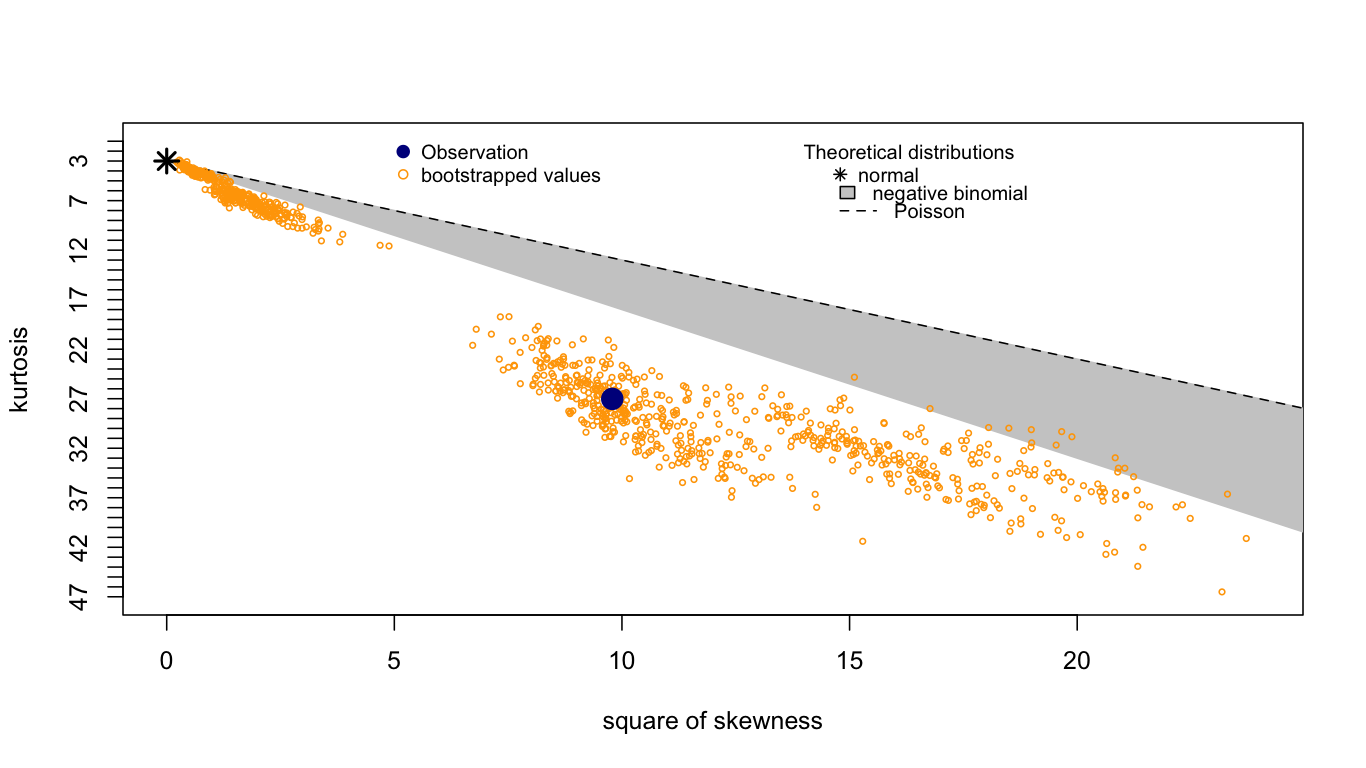
\includegraphics[width=170mm]{img/_fitofwpp}}
\caption{Cullen and Frey Graphs} \label{fig:fit}
\end{figure}

\clearpage

	\bibliography{assignment3}
	\bibliographystyle{plainnat}
	
\end{document}